\documentclass[twoside]{book}

% Packages required by doxygen
\usepackage{fixltx2e}
\usepackage{calc}
\usepackage{doxygen}
\usepackage[export]{adjustbox} % also loads graphicx
\usepackage{graphicx}
\usepackage[utf8]{inputenc}
\usepackage{makeidx}
\usepackage{multicol}
\usepackage{multirow}
\PassOptionsToPackage{warn}{textcomp}
\usepackage{textcomp}
\usepackage[nointegrals]{wasysym}
\usepackage[table]{xcolor}

% Font selection
\usepackage[T1]{fontenc}
\usepackage[scaled=.90]{helvet}
\usepackage{courier}
\usepackage{amssymb}
\usepackage{sectsty}
\renewcommand{\familydefault}{\sfdefault}
\allsectionsfont{%
  \fontseries{bc}\selectfont%
  \color{darkgray}%
}
\renewcommand{\DoxyLabelFont}{%
  \fontseries{bc}\selectfont%
  \color{darkgray}%
}
\newcommand{\+}{\discretionary{\mbox{\scriptsize$\hookleftarrow$}}{}{}}

% Page & text layout
\usepackage{geometry}
\geometry{%
  a4paper,%
  top=2.5cm,%
  bottom=2.5cm,%
  left=2.5cm,%
  right=2.5cm%
}
\tolerance=750
\hfuzz=15pt
\hbadness=750
\setlength{\emergencystretch}{15pt}
\setlength{\parindent}{0cm}
\setlength{\parskip}{0.2cm}
\makeatletter
\renewcommand{\paragraph}{%
  \@startsection{paragraph}{4}{0ex}{-1.0ex}{1.0ex}{%
    \normalfont\normalsize\bfseries\SS@parafont%
  }%
}
\renewcommand{\subparagraph}{%
  \@startsection{subparagraph}{5}{0ex}{-1.0ex}{1.0ex}{%
    \normalfont\normalsize\bfseries\SS@subparafont%
  }%
}
\makeatother

% Headers & footers
\usepackage{fancyhdr}
\pagestyle{fancyplain}
\fancyhead[LE]{\fancyplain{}{\bfseries\thepage}}
\fancyhead[CE]{\fancyplain{}{}}
\fancyhead[RE]{\fancyplain{}{\bfseries\leftmark}}
\fancyhead[LO]{\fancyplain{}{\bfseries\rightmark}}
\fancyhead[CO]{\fancyplain{}{}}
\fancyhead[RO]{\fancyplain{}{\bfseries\thepage}}
\fancyfoot[LE]{\fancyplain{}{}}
\fancyfoot[CE]{\fancyplain{}{}}
\fancyfoot[RE]{\fancyplain{}{\bfseries\scriptsize Generated on Mon Mar 7 2016 16\+:10\+:03 for Test-\/\+C++ by Doxygen }}
\fancyfoot[LO]{\fancyplain{}{\bfseries\scriptsize Generated on Mon Mar 7 2016 16\+:10\+:03 for Test-\/\+C++ by Doxygen }}
\fancyfoot[CO]{\fancyplain{}{}}
\fancyfoot[RO]{\fancyplain{}{}}
\renewcommand{\footrulewidth}{0.4pt}
\renewcommand{\chaptermark}[1]{%
  \markboth{#1}{}%
}
\renewcommand{\sectionmark}[1]{%
  \markright{\thesection\ #1}%
}

% Indices & bibliography
\usepackage{natbib}
\usepackage[titles]{tocloft}
\setcounter{tocdepth}{3}
\setcounter{secnumdepth}{5}
\makeindex

% Hyperlinks (required, but should be loaded last)
\usepackage{ifpdf}
\ifpdf
  \usepackage[pdftex,pagebackref=true]{hyperref}
\else
  \usepackage[ps2pdf,pagebackref=true]{hyperref}
\fi
\hypersetup{%
  colorlinks=true,%
  linkcolor=blue,%
  citecolor=blue,%
  unicode%
}

% Custom commands
\newcommand{\clearemptydoublepage}{%
  \newpage{\pagestyle{empty}\cleardoublepage}%
}


%===== C O N T E N T S =====

\begin{document}

% Titlepage & ToC
\hypersetup{pageanchor=false,
             bookmarks=true,
             bookmarksnumbered=true,
             pdfencoding=unicode
            }
\pagenumbering{roman}
\begin{titlepage}
\vspace*{7cm}
\begin{center}%
{\Large Test-\/\+C++ }\\
\vspace*{1cm}
{\large Generated by Doxygen 1.8.10}\\
\vspace*{0.5cm}
{\small Mon Mar 7 2016 16:10:03}\\
\end{center}
\end{titlepage}
\clearemptydoublepage
\tableofcontents
\clearemptydoublepage
\pagenumbering{arabic}
\hypersetup{pageanchor=true}

%--- Begin generated contents ---
\chapter{Hierarchical Index}
\section{Class Hierarchy}
This inheritance list is sorted roughly, but not completely, alphabetically\+:\begin{DoxyCompactList}
\item Form\begin{DoxyCompactList}
\item \contentsline{section}{Program}{\pageref{class_program}}{}
\end{DoxyCompactList}
\item \contentsline{section}{Grid$<$ result\+Type $>$}{\pageref{class_grid}}{}
\item \contentsline{section}{Mandlebrot}{\pageref{struct_mandlebrot}}{}
\item \contentsline{section}{Result\+Grid$<$ result\+Type, calculator $>$}{\pageref{class_result_grid}}{}
\end{DoxyCompactList}

\chapter{Class Index}
\section{Class List}
Here are the classes, structs, unions and interfaces with brief descriptions\+:\begin{DoxyCompactList}
\item\contentsline{section}{\hyperlink{class_grid}{Grid$<$ result\+Type $>$} \\*This class represents a two dimensional grid }{\pageref{class_grid}}{}
\item\contentsline{section}{\hyperlink{struct_mandlebrot}{Mandlebrot} \\*A functor to calculate the number of iterations before convergence of the mandlebrot sequence }{\pageref{struct_mandlebrot}}{}
\item\contentsline{section}{\hyperlink{class_program}{Program} \\*The main form where results are displayed }{\pageref{class_program}}{}
\item\contentsline{section}{\hyperlink{class_result_grid}{Result\+Grid$<$ result\+Type, calculator $>$} \\*This class hold the values of a function evaluated on a two dimensional grid }{\pageref{class_result_grid}}{}
\end{DoxyCompactList}

\chapter{Class Documentation}
\hypertarget{class_grid}{}\section{Grid$<$ result\+Type $>$ Class Template Reference}
\label{class_grid}\index{Grid$<$ result\+Type $>$@{Grid$<$ result\+Type $>$}}


This class represents a two dimensional grid.  




{\ttfamily \#include $<$Grid.\+h$>$}

\subsection*{Public Member Functions}
\begin{DoxyCompactItemize}
\item 
\hyperlink{class_grid_a3f19f2be9f0547b305c5cac906a37b33}{Grid} (int x\+Points, int y\+Points, result\+Type x0, result\+Type x\+Max, result\+Type y0, result\+Type y\+Max)
\item 
result\+Type \hyperlink{class_grid_ad700ddfc8b14513dff9766b2d80d2f3f}{X} (int i)
\item 
result\+Type \hyperlink{class_grid_a65d9b614b67a2f8cbff493835cd7b42a}{Y} (int j)
\end{DoxyCompactItemize}
\subsection*{Public Attributes}
\begin{DoxyCompactItemize}
\item 
\hypertarget{class_grid_a5ecc47a87f79457507195a9ed01705ee}{}int \hyperlink{class_grid_a5ecc47a87f79457507195a9ed01705ee}{X\+Points}\label{class_grid_a5ecc47a87f79457507195a9ed01705ee}

\begin{DoxyCompactList}\small\item\em The number of points used to represent the x-\/axis. \end{DoxyCompactList}\item 
\hypertarget{class_grid_aa36f01c184bcaf78ca18b44df5855833}{}int \hyperlink{class_grid_aa36f01c184bcaf78ca18b44df5855833}{Y\+Points}\label{class_grid_aa36f01c184bcaf78ca18b44df5855833}

\begin{DoxyCompactList}\small\item\em The number of points used to represent the y-\/axis. \end{DoxyCompactList}\end{DoxyCompactItemize}


\subsection{Detailed Description}
\subsubsection*{template$<$class result\+Type$>$class Grid$<$ result\+Type $>$}

This class represents a two dimensional grid. 


\begin{DoxyParams}{Parameters}
{\em result\+Type} & The type to return the x-\/y coordinate as. \\
\hline
\end{DoxyParams}


\subsection{Constructor \& Destructor Documentation}
\hypertarget{class_grid_a3f19f2be9f0547b305c5cac906a37b33}{}\index{Grid@{Grid}!Grid@{Grid}}
\index{Grid@{Grid}!Grid@{Grid}}
\subsubsection[{Grid(int x\+Points, int y\+Points, result\+Type x0, result\+Type x\+Max, result\+Type y0, result\+Type y\+Max)}]{\setlength{\rightskip}{0pt plus 5cm}template$<$class result\+Type $>$ {\bf Grid}$<$ result\+Type $>$\+::{\bf Grid} (
\begin{DoxyParamCaption}
\item[{int}]{x\+Points, }
\item[{int}]{y\+Points, }
\item[{result\+Type}]{x0, }
\item[{result\+Type}]{x\+Max, }
\item[{result\+Type}]{y0, }
\item[{result\+Type}]{y\+Max}
\end{DoxyParamCaption}
)}\label{class_grid_a3f19f2be9f0547b305c5cac906a37b33}
Intializes a new \hyperlink{class_grid}{Grid} instance. 
\begin{DoxyParams}{Parameters}
{\em x\+Points} & The number of points to represent the x-\/axis. \\
\hline
{\em y\+Points} & The number of points to represent the y-\/axis. \\
\hline
{\em x0} & The value of x at the zeroth point. \\
\hline
{\em x\+Max} & The value of x at the x\+Point point. \\
\hline
{\em y0} & The value of y at the zeroth point. \\
\hline
{\em y\+Max} & The value of y at the y\+Point point. \\
\hline
\end{DoxyParams}


\subsection{Member Function Documentation}
\hypertarget{class_grid_ad700ddfc8b14513dff9766b2d80d2f3f}{}\index{Grid@{Grid}!X@{X}}
\index{X@{X}!Grid@{Grid}}
\subsubsection[{X(int i)}]{\setlength{\rightskip}{0pt plus 5cm}template$<$class result\+Type $>$ result\+Type {\bf Grid}$<$ result\+Type $>$\+::X (
\begin{DoxyParamCaption}
\item[{int}]{i}
\end{DoxyParamCaption}
)}\label{class_grid_ad700ddfc8b14513dff9766b2d80d2f3f}
The value of the x-\/coordinate for the index i. 
\begin{DoxyParams}{Parameters}
{\em i} & The x-\/axis index for the wanted grid value. \\
\hline
\end{DoxyParams}
\hypertarget{class_grid_a65d9b614b67a2f8cbff493835cd7b42a}{}\index{Grid@{Grid}!Y@{Y}}
\index{Y@{Y}!Grid@{Grid}}
\subsubsection[{Y(int j)}]{\setlength{\rightskip}{0pt plus 5cm}template$<$class result\+Type $>$ result\+Type {\bf Grid}$<$ result\+Type $>$\+::Y (
\begin{DoxyParamCaption}
\item[{int}]{j}
\end{DoxyParamCaption}
)}\label{class_grid_a65d9b614b67a2f8cbff493835cd7b42a}
The value of the y-\/coordinate for the index j. 
\begin{DoxyParams}{Parameters}
{\em j} & The y-\/axis index for the wanted grid value. \\
\hline
\end{DoxyParams}


The documentation for this class was generated from the following files\+:\begin{DoxyCompactItemize}
\item 
Mandlebrot/Grid.\+h\item 
Mandlebrot/Grid.\+hxx\end{DoxyCompactItemize}

\hypertarget{struct_mandlebrot}{}\section{Mandlebrot Struct Reference}
\label{struct_mandlebrot}\index{Mandlebrot@{Mandlebrot}}


A functor to calculate the number of iterations before convergence of the mandlebrot sequence.  




{\ttfamily \#include $<$Mandlebrot.\+h$>$}

\subsection*{Public Member Functions}
\begin{DoxyCompactItemize}
\item 
\hyperlink{struct_mandlebrot_ab6d9fdcf93a8a8a396f28c8a352520a6}{Mandlebrot} (int max\+Iter)
\begin{DoxyCompactList}\small\item\em Initializes a new \hyperlink{struct_mandlebrot}{Mandlebrot} instance. \end{DoxyCompactList}\item 
int \hyperlink{struct_mandlebrot_a56d1e2fce182328322d3ebb1a78b9b90}{operator()} (std\+::complex$<$ double $>$ c)
\begin{DoxyCompactList}\small\item\em Calculate the number of iterations for f(z\+\_\+n+1) = f(z\+\_\+n)$^\wedge$2 + c, while $\vert$f(z)$\vert$$<$=2, from a complex number c. \end{DoxyCompactList}\item 
\hypertarget{struct_mandlebrot_a34f5e04a19852ac819d9be3b4057e0f3}{}int \hyperlink{struct_mandlebrot_a34f5e04a19852ac819d9be3b4057e0f3}{operator()} (double re\+C, double im\+C)\label{struct_mandlebrot_a34f5e04a19852ac819d9be3b4057e0f3}

\begin{DoxyCompactList}\small\item\em Calculate the number of iterations for f(z\+\_\+n+1) = f(z\+\_\+n)$^\wedge$2 + c, while $\vert$f(z)$\vert$$<$=2, from the real and imaginary components of c. \end{DoxyCompactList}\end{DoxyCompactItemize}


\subsection{Detailed Description}
A functor to calculate the number of iterations before convergence of the mandlebrot sequence. 

A simple escape time algorithm as described on Wikipedia is used for calculations. 

\subsection{Constructor \& Destructor Documentation}
\hypertarget{struct_mandlebrot_ab6d9fdcf93a8a8a396f28c8a352520a6}{}\index{Mandlebrot@{Mandlebrot}!Mandlebrot@{Mandlebrot}}
\index{Mandlebrot@{Mandlebrot}!Mandlebrot@{Mandlebrot}}
\subsubsection[{Mandlebrot(int max\+Iter)}]{\setlength{\rightskip}{0pt plus 5cm}Mandlebrot\+::\+Mandlebrot (
\begin{DoxyParamCaption}
\item[{int}]{max\+Iter}
\end{DoxyParamCaption}
)}\label{struct_mandlebrot_ab6d9fdcf93a8a8a396f28c8a352520a6}


Initializes a new \hyperlink{struct_mandlebrot}{Mandlebrot} instance. 

Initialization consists of setting the maximun number of iterations. 

\subsection{Member Function Documentation}
\hypertarget{struct_mandlebrot_a56d1e2fce182328322d3ebb1a78b9b90}{}\index{Mandlebrot@{Mandlebrot}!operator()@{operator()}}
\index{operator()@{operator()}!Mandlebrot@{Mandlebrot}}
\subsubsection[{operator()(std\+::complex$<$ double $>$ c)}]{\setlength{\rightskip}{0pt plus 5cm}int Mandlebrot\+::operator() (
\begin{DoxyParamCaption}
\item[{std\+::complex$<$ double $>$}]{c}
\end{DoxyParamCaption}
)}\label{struct_mandlebrot_a56d1e2fce182328322d3ebb1a78b9b90}


Calculate the number of iterations for f(z\+\_\+n+1) = f(z\+\_\+n)$^\wedge$2 + c, while $\vert$f(z)$\vert$$<$=2, from a complex number c. 

The initial 

The documentation for this struct was generated from the following files\+:\begin{DoxyCompactItemize}
\item 
Mandlebrot/Mandlebrot.\+h\item 
Mandlebrot/Mandlebrot.\+cpp\end{DoxyCompactItemize}

\hypertarget{class_program}{}\section{Program Class Reference}
\label{class_program}\index{Program@{Program}}


The main form where results are displayed.  




{\ttfamily \#include $<$Program.\+h$>$}

Inheritance diagram for Program\+:\begin{figure}[H]
\begin{center}
\leavevmode
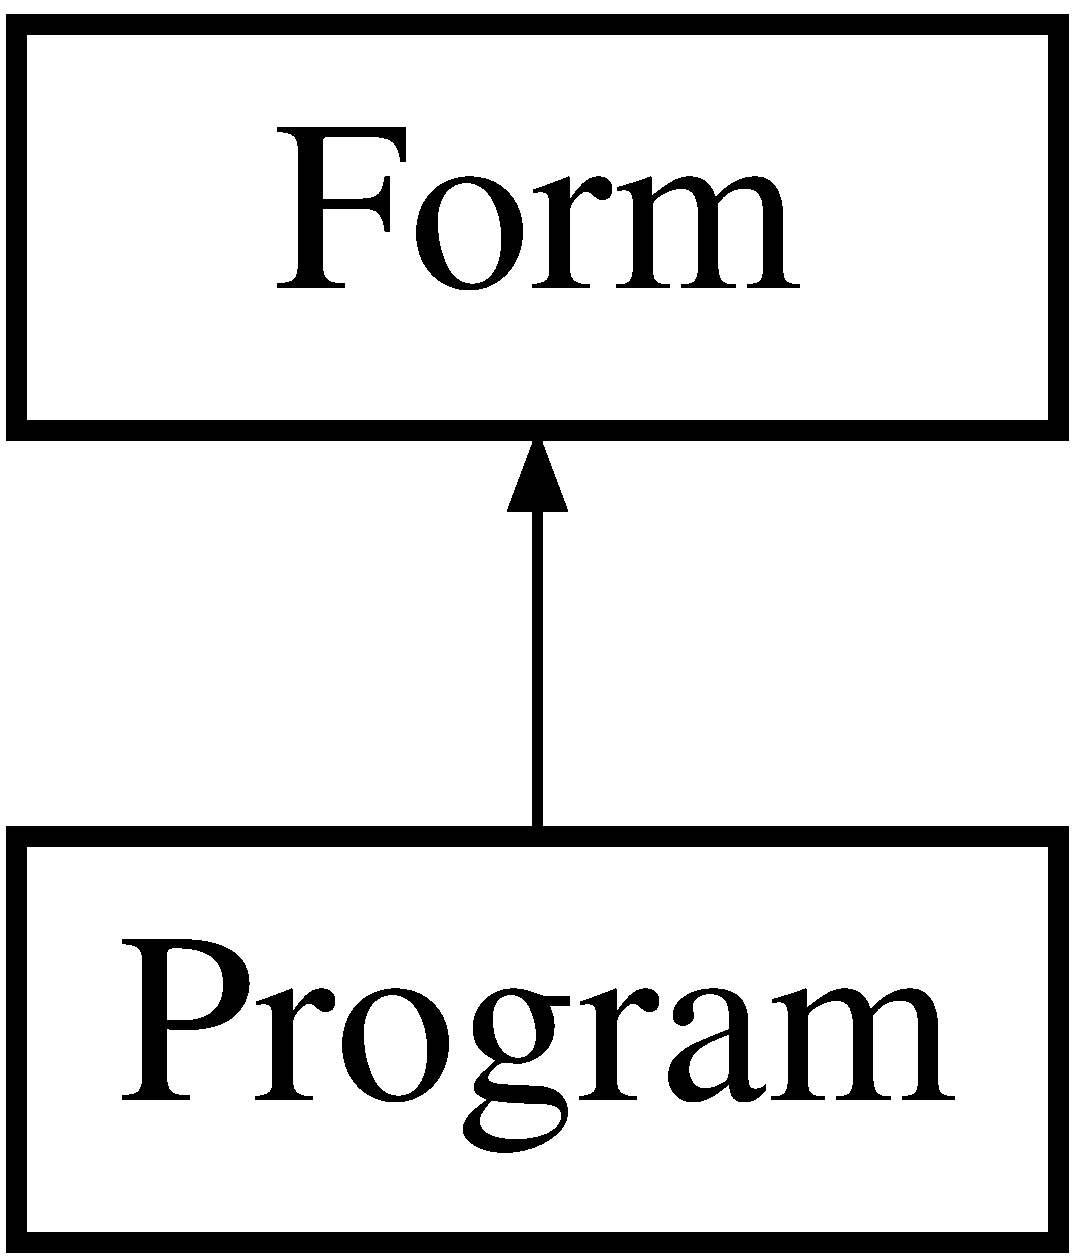
\includegraphics[height=2.000000cm]{class_program}
\end{center}
\end{figure}
\subsection*{Public Member Functions}
\begin{DoxyCompactItemize}
\item 
\hyperlink{class_program_aaefaa0df08f3484476fc4d61e97acbdc}{Program} ()
\begin{DoxyCompactList}\small\item\em Intializes the \hyperlink{class_program}{Program} class. \end{DoxyCompactList}\end{DoxyCompactItemize}


\subsection{Detailed Description}
The main form where results are displayed. 

This form displays the results of the mandlebrot calculation drawn onto a .Net Picture\+Box element. 

\subsection{Constructor \& Destructor Documentation}
\hypertarget{class_program_aaefaa0df08f3484476fc4d61e97acbdc}{}\index{Program@{Program}!Program@{Program}}
\index{Program@{Program}!Program@{Program}}
\subsubsection[{Program()}]{\setlength{\rightskip}{0pt plus 5cm}Program\+::\+Program (
\begin{DoxyParamCaption}
{}
\end{DoxyParamCaption}
)}\label{class_program_aaefaa0df08f3484476fc4d61e97acbdc}


Intializes the \hyperlink{class_program}{Program} class. 

Sets the form\textquotesingle{}s text, bounds and resize handler. Also initalizates the color palete and adds a picture box control. 

The documentation for this class was generated from the following files\+:\begin{DoxyCompactItemize}
\item 
Mandlebrot/Program.\+h\item 
Mandlebrot/Program.\+cpp\end{DoxyCompactItemize}

\hypertarget{class_result_grid}{}\section{Result\+Grid$<$ result\+Type, calculator $>$ Class Template Reference}
\label{class_result_grid}\index{Result\+Grid$<$ result\+Type, calculator $>$@{Result\+Grid$<$ result\+Type, calculator $>$}}


This class hold the values of a function evaluated on a two dimensional grid.  




{\ttfamily \#include $<$Result\+Grid.\+h$>$}

\subsection*{Public Member Functions}
\begin{DoxyCompactItemize}
\item 
\hyperlink{class_result_grid_a9ba2da6df1f07b6a96250376ed89094d}{Result\+Grid} (\hyperlink{class_grid}{Grid}$<$ double $>$ grid, calculator calc)
\item 
result\+Type \hyperlink{class_result_grid_ac9bb7d6af4293ac18302e3e895f00081}{Point} (int i, int j)
\end{DoxyCompactItemize}
\subsection*{Public Attributes}
\begin{DoxyCompactItemize}
\item 
\hypertarget{class_result_grid_ac20f44d6320de3f28e8b9041fa8a0a5e}{}int \hyperlink{class_result_grid_ac20f44d6320de3f28e8b9041fa8a0a5e}{X\+Points}\label{class_result_grid_ac20f44d6320de3f28e8b9041fa8a0a5e}

\begin{DoxyCompactList}\small\item\em The number of points used to represent the x-\/axis. \end{DoxyCompactList}\item 
\hypertarget{class_result_grid_af0886625e1133e4fe7d72c04a472ff67}{}int \hyperlink{class_result_grid_af0886625e1133e4fe7d72c04a472ff67}{Y\+Points}\label{class_result_grid_af0886625e1133e4fe7d72c04a472ff67}

\begin{DoxyCompactList}\small\item\em The number of points used to represent the y-\/axis. \end{DoxyCompactList}\end{DoxyCompactItemize}


\subsection{Detailed Description}
\subsubsection*{template$<$class result\+Type, class calculator$>$class Result\+Grid$<$ result\+Type, calculator $>$}

This class hold the values of a function evaluated on a two dimensional grid. 


\begin{DoxyParams}{Parameters}
{\em result\+Type} & The return type of the calculator functor. \\
\hline
{\em calculator} & T\+He type of the functor passed in the constructor. \\
\hline
\end{DoxyParams}


\subsection{Constructor \& Destructor Documentation}
\hypertarget{class_result_grid_a9ba2da6df1f07b6a96250376ed89094d}{}\index{Result\+Grid@{Result\+Grid}!Result\+Grid@{Result\+Grid}}
\index{Result\+Grid@{Result\+Grid}!Result\+Grid@{Result\+Grid}}
\subsubsection[{Result\+Grid(\+Grid$<$ double $>$ grid, calculator calc)}]{\setlength{\rightskip}{0pt plus 5cm}template$<$class result\+Type , class calculator $>$ {\bf Result\+Grid}$<$ result\+Type, calculator $>$\+::{\bf Result\+Grid} (
\begin{DoxyParamCaption}
\item[{{\bf Grid}$<$ double $>$}]{grid, }
\item[{calculator}]{calc}
\end{DoxyParamCaption}
)}\label{class_result_grid_a9ba2da6df1f07b6a96250376ed89094d}
Initializes a \hyperlink{class_result_grid}{Result\+Grid} instance. 
\begin{DoxyParams}{Parameters}
{\em grid} & The grid to evaluate the function at. \\
\hline
{\em calc} & The functor from which to calcuate function values. \\
\hline
\end{DoxyParams}


\subsection{Member Function Documentation}
\hypertarget{class_result_grid_ac9bb7d6af4293ac18302e3e895f00081}{}\index{Result\+Grid@{Result\+Grid}!Point@{Point}}
\index{Point@{Point}!Result\+Grid@{Result\+Grid}}
\subsubsection[{Point(int i, int j)}]{\setlength{\rightskip}{0pt plus 5cm}template$<$class result\+Type , class calculator $>$ result\+Type {\bf Result\+Grid}$<$ result\+Type, calculator $>$\+::Point (
\begin{DoxyParamCaption}
\item[{int}]{i, }
\item[{int}]{j}
\end{DoxyParamCaption}
)}\label{class_result_grid_ac9bb7d6af4293ac18302e3e895f00081}
The value of a function at the indecies i and j. 
\begin{DoxyParams}{Parameters}
{\em i} & The x-\/axis index for the wanted value. \\
\hline
{\em j} & The y-\/axis index for the wanted value. \\
\hline
\end{DoxyParams}


The documentation for this class was generated from the following files\+:\begin{DoxyCompactItemize}
\item 
Mandlebrot/Result\+Grid.\+h\item 
Mandlebrot/Result\+Grid.\+hxx\end{DoxyCompactItemize}

%--- End generated contents ---

% Index
\backmatter
\newpage
\phantomsection
\clearemptydoublepage
\addcontentsline{toc}{chapter}{Index}
\printindex

\end{document}
